\section{Methodology}
\label{sec:methodology}

This section specifies the author-resolution method at the level needed to reproduce it. Every constant below was read from the committed configuration and code. The weights and thresholds are engineering defaults chosen by the developers. They were not learned from data, and they have not been calibrated or validated against independent labels.

\subsection{Task Definition}
\label{sec:task}
A \emph{query} $q=(n,\kappa)$ is a printed author name $n$ with an optional context $\kappa$ (Section~\ref{sec:leakage}). The \emph{provider catalog} is the set of author profiles in OpenAlex. A \emph{candidate} is a provider profile returned for $q$, and the \emph{candidate pool} $C(q)=(c_1,\dots,c_m)$, $m\le 10$, is the ordered list the provider returns. The \emph{expected identity} $g(q)$ is the person the query is meant to denote. It is defined by the benchmark's identity group and is provisional until audited (Section~\ref{sec:design}). A profile is \emph{mapped} to $g(q)$ if it represents that person, and a person may be mapped to several profiles because providers fragment identities.

Five operations are kept separate. \emph{Candidate retrieval} produces $C(q)$. \emph{Candidate ranking} orders $C(q)$ by a heuristic score. \emph{Identity assignment} selects one candidate as the answer. \emph{Abstention} withholds assignment and routes the query to \emph{manual review} when some candidate is plausible, or leaves it \emph{unresolved} when none is. A provider failure produces no decision at all. The unit of analysis is the query, with one primary query per identity group. Queries from the same name block are not independent observations (Section~\ref{sec:design}).

\subsection{Candidate Retrieval Configurations}
\label{sec:retrieval}
Two retrieval configurations are defined. Both request one page of at most ten profiles from the OpenAlex authors endpoint.

\textbf{R0} sends the trimmed raw query as \texttt{filter=display\_name.search:}$n$. It applies no normalization and no fallback. R0 exists only in the capture toolkit; the application never issues it.

\textbf{R2} is the application's committed strategy. It first applies the query cleaner, which normalizes Unicode (NFC), collapses whitespace, and joins ``Le'' or ``La'' to a following capitalized alphabetic token of more than two letters (for example ``Le Cun'' becomes ``LeCun''), and then sends the same filter. If, and only if, that primary request succeeds with no valid candidate and the cleaned query contains an initial (a single letter followed by a period), a second request uses \texttt{search=}$n$, a broader provider search, and appends identifiers not yet seen. The capture toolkit records the primary and fallback outcomes of R2 separately. The application's own fallback code swallows a failed fallback request, so there a failed fallback can end as an empty pool; this known defect was not changed. The application also refuses inputs that look like institution names before any request, which the toolkit's R2 does not do.

The two configurations therefore differ only in query text and in the fallback. They issue identical requests whenever cleaning leaves the query unchanged and no fallback applies, and the toolkit then stores one physical response and shares it between them. A shared response is one provider observation used by two logical configurations, and not two independent observations. In the 50-case smoke capture (Section~\ref{sec:smoke}) the two configurations issued identical primary requests in all fifty cases, so query cleaning changed no request, and the only difference was the fallback after two successful empty R0 responses. These are descriptive smoke observations about that sample. They provide no meaningful comparative test of the two strategies, and neither configuration is described as better than the other.

\subsection{Evidence Signals}
\label{sec:signals}
The resolver implements five extractors, but not all five take part in the LAGOS-AND experiment. Name similarity is always available. Institutional and temporal evidence are available where the query context and the candidate profile carry the metadata. Publication overlap is observed only in the exploratory condition C1x and is excluded from the primary condition C1. Coauthor evidence is unavailable, so the effective signal set has at most four members (Table~\ref{tab:availability}).

\begin{table}[t]
\caption{Availability of the five signals in the LAGOS-AND experiment.}
\label{tab:availability}
\centering
\footnotesize
\renewcommand{\arraystretch}{1.1}
\begin{tabular}{@{}p{0.27\columnwidth}p{0.62\columnwidth}@{}}
\toprule
\textbf{Signal} & \textbf{Availability} \\
\midrule
Name similarity & Available \\
Institutional evidence & Where the query and the candidate both carry affiliation data \\
Publication overlap & C1x only (exploratory); not in primary C1 \\
Coauthor evidence & Unavailable: coauthors are name strings without identifiers \\
Temporal evidence & Where the candidate has yearly counts \\
\bottomrule
\end{tabular}
\end{table}

For each candidate $c$, each implemented extractor returns a score $e_k(c)\in[0,1]$ or declares the signal unavailable. Table~\ref{tab:signals} summarizes them. Weights $w_k$ are the defaults 0.35, 0.25, 0.20, 0.10 and 0.10 in the order shown.

\begin{table*}[t]
\caption{Evidence signals: default weight, inputs and computation. ``Unavailable'' signals are omitted from scoring; they are never scored as zero or as agreement.}
\label{tab:signals}
\centering
\footnotesize
\renewcommand{\arraystretch}{1.12}
\begin{tabular}{@{}p{0.09\textwidth}p{0.04\textwidth}p{0.20\textwidth}p{0.30\textwidth}p{0.25\textwidth}@{}}
\toprule
\textbf{Signal} & \textbf{$w_k$} & \textbf{Inputs (query; candidate)} & \textbf{Score $e_k$} & \textbf{Unavailable when} \\
\midrule
Name similarity & 0.35 & Query name and aliases; display name and aliases & Token-sort ratio of casefolded, whitespace-collapsed names, divided by 100; maximum over all name pairs. No diacritic folding or transliteration & No query name or no candidate name \\
Institutional evidence & 0.25 & Institution name, OpenAlex ID or ROR ID; last known institutions and affiliations & For each pair: ROR identifiers equal 1, different 0; else OpenAlex IDs equal 1, different 0; else token-sort ratio of names. Maximum over pairs & No institution supplied, no candidate affiliation, or no pair comparable \\
Publication overlap & 0.20 & DOIs or OpenAlex work IDs (titles ignored); authorships of those works & Supplied works that list the candidate as an author, divided by supplied works that could be compared (found, author list not truncated) & No publication identifiers, retrieval failed or not performed, or none comparable \\
Coauthor evidence & 0.10 & OpenAlex coauthor \emph{author IDs} only; coauthors from a bounded sample of the candidate's works & Matched IDs divided by the smaller of the supplied IDs and the candidate's coauthors. Names are never scored & Names only, no sample, retrieval failed, or no overlap in an incomplete sample \\
Temporal evidence & 0.10 & Active-year range; first and last year in the profile's yearly counts & Overlap in years divided by the shorter of the two ranges; zero if the query range follows the candidate range & No query range or candidate range, or the query range precedes the candidate range (inconclusive) \\
\bottomrule
\end{tabular}
\end{table*}

Each signal ends in a status, namely \emph{observed} (a score exists, and 0 means observed non-support) or one of several \emph{unavailable} states: query input absent, candidate data absent, not retrieved, retrieval failed, inconclusive, or input not comparable. The status, the raw comparison values and the provenance are stored with the score. Because a missing signal says nothing about the candidate, it is omitted and the remaining weights are renormalized. With $A(c)$ the set of observed signals,
\begin{equation}
s(c)=\frac{\sum_{k\in A(c)} w_k\,e_k(c)}{\sum_{k\in A(c)} w_k},
\label{eq:score}
\end{equation}
and $s(c)$ is undefined if $A(c)=\emptyset$. The effective weight of signal $k$ is $w_k/\sum_{j\in A(c)}w_j$ and is stored with the score.

Candidates are ordered by $s(c)$ in descending order, undefined scores last, with ties broken by descending provider identifier. The ordering is deterministic and is not an identity assertion.

Two properties limit what the score means. First, $s(c)$ is a heuristic. It is not a probability, and the weights are not calibrated. Second, candidates in one pool may be scored over different signal sets $A(c)$, and a renormalized score over two signals is not on the same footing as one over four. Their scores are therefore not necessarily comparable, and this affects the ranking, the margin and the forced top-one baseline. We add no common-subset re-ranking and no new formula. The signal set of every candidate is reported with every result.

\subsection{Decision Policy}
\label{sec:policy}
Let $c_1$ be the top-ranked candidate with score $s_1$, and $s_2$ the score of the best-ranked competitor that has a score. The margin is $\Delta=s_1-s_2$ and the dominance ratio is $\rho=s_1/s_2$, which is not evaluated when $s_2=0$. The numerical gates are $\tau_a=0.75$ (automatic score), $\tau_\Delta=0.15$ (margin), $\tau_\rho=1.35$ (dominance), $\tau_m=0.45$ (manual-review score) and a minimum of two observed signals for the top candidate. They are environment-overridable defaults, and the effective values are recorded in every run manifest. Table~\ref{tab:gates} lists the rules, and Fig.~\ref{fig:methodology} shows the flow.

\begin{table}[t]
\caption{Decision rules. A query is assigned automatically only if every gate passes and no safeguard applies. The identifiers follow the protocol and the policy module.}
\label{tab:gates}
\centering
\footnotesize
\renewcommand{\arraystretch}{1.1}
\begin{tabular}{@{}p{0.052\columnwidth}p{0.68\columnwidth}p{0.15\columnwidth}@{}}
\toprule
\textbf{Rule} & \textbf{Condition} & \textbf{Protocol} \\
\midrule
G0 & $s_1$ undefined: category ``no score'' (stored as unresolved with a reason) & P0 \\
G1 & $s_1\ge\tau_a$ and at least two observed signals for $c_1$ & P1 \\
G2 & With competitors: $\Delta\ge\tau_\Delta$ and, if $s_2>0$, $\rho\ge\tau_\rho$, computed against the best scored competitor; if no competitor has a score the gate fails & P2 \\
G3 & Single-candidate pool: G2 is waived; G1 and all safeguards still apply & P3 \\
B1 & At least one competitor has no score, even if another competitor is scored & P4 \\
B2 & $c_1$ has no observed, non-zero institution, publication or coauthor signal & P5 \\
B3 & $c_1$ has an observed signal equal to 0 & P6 \\
B4 & A scored competitor used a different signal set than $c_1$ & P7 \\
B5 & An enrichment request failed, or a candidate could not be read & P8 \\
M & Not automatic and $s_1\ge\tau_m$: manual review; otherwise unresolved & P9 \\
F & Provider failure: no decision. Successful empty pool: stored as unresolved with reason ``empty retrieval''. Both are reported as separate categories & P10 \\
\bottomrule
\end{tabular}
\end{table}

\begin{figure*}[t]
\centering
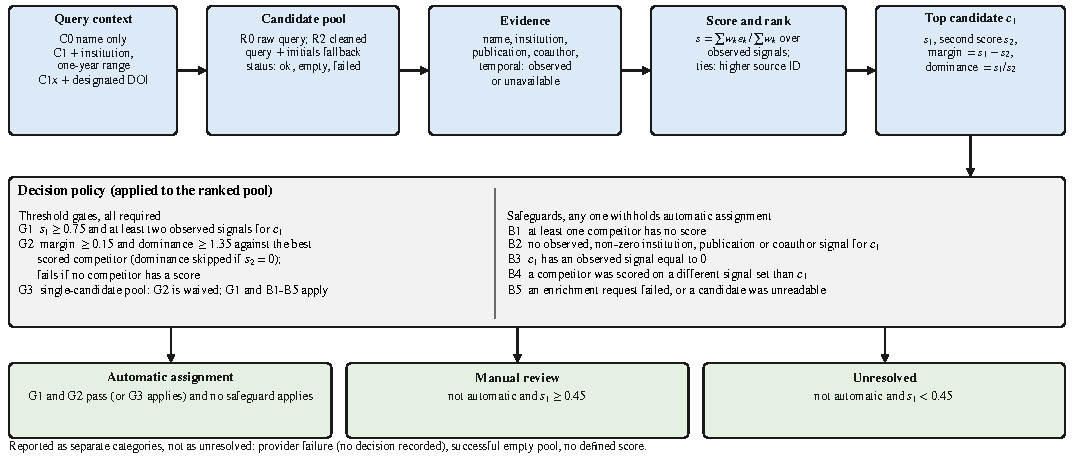
\includegraphics[width=\textwidth]{figures/methodology.pdf}
\caption{Author-resolution methodology. The decision policy (G1--G3 and B1--B5 of Table~\ref{tab:gates}) is applied to the ranked pool and yields one of three outcomes. Failed and empty pools bypass the policy. Regenerate with \texttt{figures/make\_figures.py}.}
\label{fig:methodology}
\end{figure*}

A high score is not enough for automatic assignment, for three reasons. The score is renormalized, so a score of 1.0 over a single signal is possible, and the policy requires at least two observed signals. Name agreement is common among different people, so B2 requires an observed, non-zero institution, publication or coauthor signal, and name together with temporal agreement is not sufficient. These two requirements together make automatic assignment structurally impossible when only the name is supplied: coverage is zero by design in that setting, which is a property of the policy and not evidence that the policy is safe or accurate. Third, a score can be inflated by missing evidence, and B1, B4 and B5 withhold automation when competitors were not scored comparably or evidence retrieval was incomplete. Safeguards B1 to B5 only withhold automation and route the query to manual review. None introduces a new numeric threshold, and their effect on precision and coverage has not been measured.

Three policies are applied to the same frozen pool and evidence in the experiments. The \emph{full selective policy} (artifact identifier \texttt{selective\_policy\_v2}) applies every rule of Table~\ref{tab:gates}. The \emph{threshold-gate ablation with P3 relaxation} (artifact identifier \texttt{legacy\_gates\_plus\_p3}) applies G0 to G3 and the manual-review and failure rules but not the safeguard blockers B1 to B5. It is computed offline from the same snapshot and shows what the blockers change. It is not a complete removal of equivalent protections: the margin gate G2 still requires a scored competitor, so a pool whose competitors are all unscored cannot be assigned automatically. An unscored competitor next to a scored one is, however, no longer blocked, because the margin is computed against the scored one. The \emph{forced top-one policy} (\texttt{forced\_top1}) selects $c_1$ whenever $s_1$ is defined, with no abstention. The application also attaches a High, Medium or Low display label derived from the same two score thresholds; it is a user-interface convenience, is not calibrated, and is not used in any evaluation.

Six outcome categories are kept separate in every table: automatic assignment, manual review, unresolved, successful empty retrieval, provider failure, and no candidate with a defined score. A provider failure is not an unresolved identity decision. In the application's stored status, an empty pool and a pool without a defined score both appear as unresolved with a reason, and a provider failure records no resolution; the evaluation reports each as its own category. Failure handling follows from the principle that missing evidence is not negative evidence. A candidate whose stored payload cannot be parsed is dropped from the ranking, the pool is marked incomplete, and B5 withholds automatic assignment. Enrichment failures mark the affected signal unavailable and also trigger B5.

\subsection{Context Conditions and Leakage Controls}
\label{sec:leakage}
The context $\kappa$ determines which signals can be observed. Three conditions are defined (Table~\ref{tab:conditions}). \textbf{C0} supplies the name only. \textbf{C1} adds an institution and an active-year range. In the LAGOS-AND experiment it supplies no publication identifiers, so publication overlap is excluded from the primary condition. \textbf{C1x} additionally supplies publication identifiers whose independence from the gold evidence is not established.

Every DOI used in a benchmark is registered with one of three purposes. \texttt{gold\_evidence} marks a DOI used to establish the expected identity, \texttt{query\_context} marks one chosen independently of the gold evidence and eligible for the query context, and \texttt{both} marks one that serves both roles and requires a written justification. DOIs registered as \texttt{gold\_evidence} are removed from C1. DOIs registered as \texttt{both} contribute only to C1x. Publication-overlap results that rely on a leakage-prone DOI are therefore exploratory by construction. Query contexts are derived from a frozen seed and the register and are never edited after candidates have been generated; a change creates a new dataset version. C1x is reported separately and is never mixed into the primary evaluation.

\begin{table}[t]
\caption{Context conditions. Only C1 supports primary claims.}
\label{tab:conditions}
\centering
\footnotesize
\renewcommand{\arraystretch}{1.1}
\begin{tabular}{@{}p{0.10\columnwidth}p{0.55\columnwidth}p{0.24\columnwidth}@{}}
\toprule
\textbf{Cond.} & \textbf{Context supplied} & \textbf{Status} \\
\midrule
C0 & Name only & Control; automatic coverage zero by design \\
C1 & C0 plus institution and active-year range; no publication identifiers & Primary \\
C1x & C1 plus publication identifiers not shown to be independent of gold evidence & Exploratory only \\
\bottomrule
\end{tabular}
\end{table}

Coauthor evidence has a further constraint in this study. The benchmark gives coauthors as name strings without identifiers, and names are not scored, so coauthor evidence is unavailable in every condition and the effective signal set has at most four members.
